\tikzset{every picture/.style={line width=0.75pt}} %set default line width to 0.75pt        

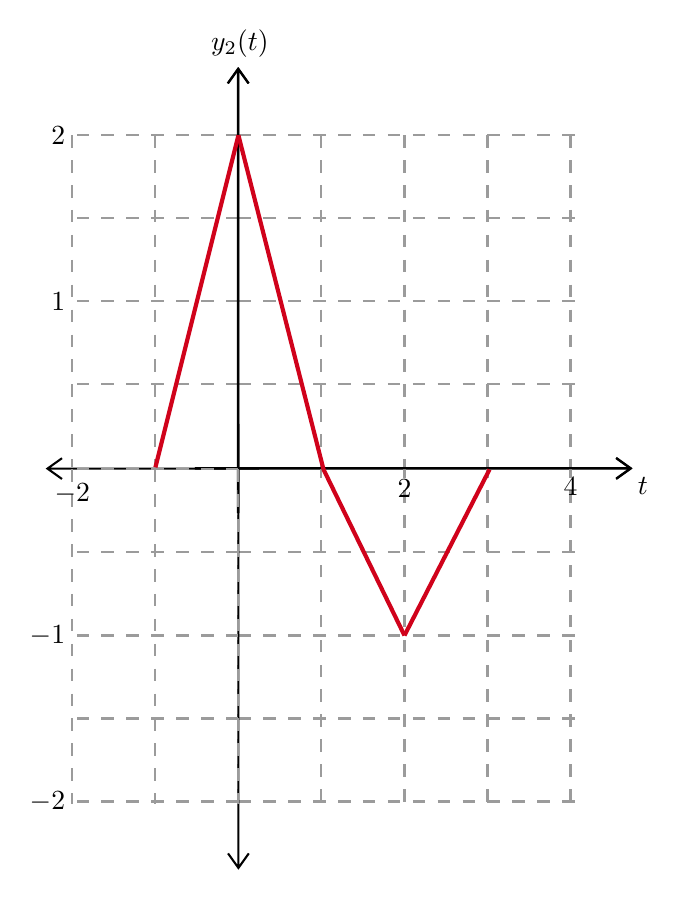
\begin{tikzpicture}[x=0.75pt,y=0.75pt,yscale=-1,xscale=1]
%uncomment if require: \path (0,757); %set diagram left start at 0, and has height of 757

%Shape: Grid [id:dp1199375004666744] 
\draw  [draw opacity=0][dash pattern={on 4.5pt off 4.5pt}] (235,131) -- (397,131) -- (397,291) -- (235,291) -- cycle ; \draw  [color={rgb, 255:red, 155; green, 155; blue, 155 }  ,draw opacity=1 ][dash pattern={on 4.5pt off 4.5pt}] (235,131) -- (235,291)(275,131) -- (275,291)(315,131) -- (315,291)(355,131) -- (355,291)(395,131) -- (395,291) ; \draw  [color={rgb, 255:red, 155; green, 155; blue, 155 }  ,draw opacity=1 ][dash pattern={on 4.5pt off 4.5pt}] (235,131) -- (397,131)(235,171) -- (397,171)(235,211) -- (397,211)(235,251) -- (397,251) ; \draw  [color={rgb, 255:red, 155; green, 155; blue, 155 }  ,draw opacity=1 ][dash pattern={on 4.5pt off 4.5pt}]  ;
%Shape: Axis 2D [id:dp9049348521282261] 
\draw  (214,291.6) -- (424,291.6)(235,99) -- (235,313) (417,286.6) -- (424,291.6) -- (417,296.6) (230,106) -- (235,99) -- (240,106)  ;
%Shape: Grid [id:dp38260027148349784] 
\draw  [draw opacity=0][dash pattern={on 4.5pt off 4.5pt}] (235,131) -- (153,131) -- (153,291) -- (235,291) -- cycle ; \draw  [color={rgb, 255:red, 155; green, 155; blue, 155 }  ,draw opacity=1 ][dash pattern={on 4.5pt off 4.5pt}] (235,131) -- (235,291)(195,131) -- (195,291)(155,131) -- (155,291) ; \draw  [color={rgb, 255:red, 155; green, 155; blue, 155 }  ,draw opacity=1 ][dash pattern={on 4.5pt off 4.5pt}] (235,131) -- (153,131)(235,171) -- (153,171)(235,211) -- (153,211)(235,251) -- (153,251) ; \draw  [color={rgb, 255:red, 155; green, 155; blue, 155 }  ,draw opacity=1 ][dash pattern={on 4.5pt off 4.5pt}]  ;
%Shape: Axis 2D [id:dp509145843401392] 
\draw  (245,291.6) -- (143,291.6)(234.8,99) -- (234.8,313) (150,286.6) -- (143,291.6) -- (150,296.6) (239.8,106) -- (234.8,99) -- (229.8,106)  ;
%Shape: Grid [id:dp3116070310441251] 
\draw  [draw opacity=0][dash pattern={on 4.5pt off 4.5pt}] (235,452) -- (397,452) -- (397,292) -- (235,292) -- cycle ; \draw  [color={rgb, 255:red, 155; green, 155; blue, 155 }  ,draw opacity=1 ][dash pattern={on 4.5pt off 4.5pt}] (235,452) -- (235,292)(275,452) -- (275,292)(315,452) -- (315,292)(355,452) -- (355,292)(395,452) -- (395,292) ; \draw  [color={rgb, 255:red, 155; green, 155; blue, 155 }  ,draw opacity=1 ][dash pattern={on 4.5pt off 4.5pt}] (235,452) -- (397,452)(235,412) -- (397,412)(235,372) -- (397,372)(235,332) -- (397,332) ; \draw  [color={rgb, 255:red, 155; green, 155; blue, 155 }  ,draw opacity=1 ][dash pattern={on 4.5pt off 4.5pt}]  ;
%Shape: Axis 2D [id:dp9445758822579701] 
\draw  (214,291.4) -- (424,291.4)(235,484) -- (235,270) (417,296.4) -- (424,291.4) -- (417,286.4) (230,477) -- (235,484) -- (240,477)  ;
%Straight Lines [id:da09039927216219223] 
\draw [color={rgb, 255:red, 208; green, 2; blue, 27 }  ,draw opacity=1 ][line width=1.5]    (195,291) -- (235,131) ;
%Straight Lines [id:da9718155597929978] 
\draw [color={rgb, 255:red, 208; green, 2; blue, 27 }  ,draw opacity=1 ][line width=1.5]    (235,131) -- (276,292) ;
%Straight Lines [id:da4117833381221786] 
\draw [color={rgb, 255:red, 208; green, 2; blue, 27 }  ,draw opacity=1 ][line width=1.5]    (276,292) -- (315,372) ;
%Shape: Grid [id:dp7431999536611184] 
\draw  [draw opacity=0][dash pattern={on 4.5pt off 4.5pt}] (235,292) -- (153,292) -- (153,453) -- (235,453) -- cycle ; \draw  [color={rgb, 255:red, 155; green, 155; blue, 155 }  ,draw opacity=1 ][dash pattern={on 4.5pt off 4.5pt}] (235,292) -- (235,453)(195,292) -- (195,453)(155,292) -- (155,453) ; \draw  [color={rgb, 255:red, 155; green, 155; blue, 155 }  ,draw opacity=1 ][dash pattern={on 4.5pt off 4.5pt}] (235,292) -- (153,292)(235,332) -- (153,332)(235,372) -- (153,372)(235,412) -- (153,412)(235,452) -- (153,452) ; \draw  [color={rgb, 255:red, 155; green, 155; blue, 155 }  ,draw opacity=1 ][dash pattern={on 4.5pt off 4.5pt}]  ;
%Straight Lines [id:da43129718422211005] 
\draw [color={rgb, 255:red, 208; green, 2; blue, 27 }  ,draw opacity=1 ][line width=1.5]    (356,292) -- (315,372) ;

% Text Node
\draw (235.72,95) node [anchor=south] [inner sep=0.75pt]    {$y_{2}( t)$};
% Text Node
\draw (426,294.4) node [anchor=north west][inner sep=0.75pt]    {$t$};
% Text Node
\draw (395,294.4) node [anchor=north] [inner sep=0.75pt]    {$4$};
% Text Node
\draw (315,295.4) node [anchor=north] [inner sep=0.75pt]    {$2$};
% Text Node
\draw (153,211) node [anchor=east] [inner sep=0.75pt]    {$1$};
% Text Node
\draw (153,131) node [anchor=east] [inner sep=0.75pt]    {$2$};
% Text Node
\draw (155,297.4) node [anchor=north] [inner sep=0.75pt]    {$-2$};
% Text Node
\draw (153,372) node [anchor=east] [inner sep=0.75pt]    {$-1$};
% Text Node
\draw (153,452) node [anchor=east] [inner sep=0.75pt]    {$-2$};


\end{tikzpicture}
